
%***********************************************************************

% This is a template to be used for the preparation of
% papers submitted to the 34th International Workshop on
% Statistical Modelling, to be held in Trieste, Italy,
% July 18-22, 2022.

% Please follow the following general guidelines:
%
% (1) Do not specify any definitions, commands or style parameters.
%     Upon submission, your file will be checked for presence of
%     \newcommand or \def statements and if found, error message will be reported
%     by the submission form.
%
% (2) Follow the template below very tightly.
%
% (3) Include .pdf figures using the \includegraphics
%      command, an example of which are given below.
%
% (4) Use file names which begin with the surname of the first author.
%
% (5) When creating labels for cross-references, please start always
%     by surname of the first author, e.g., \label{smith:likelihood}
%
% (6) The template below contains some example materials
%      to guide you through the preparation of your paper.  However,
%      remove all the redundant material from your final document
%      before submitting.

% The guidelines above are needed in order to be able to combine all
% the papers into a single proceedings book of acceptable quality.
% Please follow the guidelines as strictly as possible. Deviations may
% result in papers being either refused by the registration form
% or sent back to the authors with the request to change
% their documents according to the guidelines.

% Special characters:
% Please do not use special characters (e.g., accents).
% Use TeX composition instead, such as \~n, \'a, \`e, \v{s}, \r{u} etc.

% Changes as of IWSM 2013:
%  * \usepackage{booktabs} added which allows \toprule et al. in the tabular environment
%    (\hline\hline is not longer used)
%  * '^\T' added in iwsm.sty to denote transposed vectors and matrices within math (see example below)
%  * \usepackage{amsmath, amssymb} introduced since IWSM 2012 is allowed (allowing usage of boldsymbols
%    and other handy constructions (align, pmatrix etc.) within math)
%  * \usepackage{psfrag} introduced since IWSM 2012 is NOT allowed
%
%

%***********************************************************************
% PLEASE LEAVE THIS PART UNCHANGED
%***********************************************************************

\documentclass[twoside]{report}
\usepackage{iwsm}
\usepackage{graphicx}
\usepackage{amsmath, amssymb}
\usepackage{booktabs}
\usepackage{multirow}
% Please do not specify any new definitions, any new commands,
% and do not specify any style parameters.
% The preamble of the document should be left unchanged.

\begin{document}

%***********************************************************************
% PLEASE INSERT YOUR CONTENT FROM HERE
%***********************************************************************

% Title and running title to be used as left header:
\title{Estimated Covid-19 burden in Spain: ARCH underreported non-stationary time series}
\titlerunning{Estimated Covid-19 burden in Spain}

% Authors and running list of authors to be used as right header:
\author{David Mori\~na\inst{1}, Amanda Fern\'andez-Fontelo\inst{2}, Alejandra Caba\~na\inst{2},
Argimiro Arratia\inst{3}, Pedro Puig\inst{2}}
\authorrunning{Mori\~na et al.}     %% use \authorrunning{Surname 1} if only 1 author
                                    %% use \authorrunning{Surname 1 and Surname2} if two authors
                                    %% use \authorrunning{Surname 1 et al.} if more than two authors

% Institutes of all authors
% Include city and country of each institute, do not include the full address.
\institute{Universitat de Barcelona, Barcelona, Spain
\and Universitat Aut\`onoma de Barcelona, Cerdanyola del Vall\`es, Spain
\and Universitat Polit\`ecnica de Catalunya, Barcelona, Spain}

% E-mail of presenting author for correspondence
\email{dmorina@ub.edu}

% Brief abstract of the paper:
\abstract{The problem of dealing with misreported data is very common in a wide range of contexts. The current situation caused by the Covid-19 worldwide pandemic is a clear example, where the data provided by official sources were not always reliable due to data collection issues and to the large proportion of asymptomatic cases. In this work, we explore the performance of Bayesian Synthetic Likelihood to estimate the parameters of a model capable of dealing with misreported information and to reconstruct the most likely evolution of the phenomenon.}

% Keywords (at most 5):
\keywords{under-reported data; ARCH models; infectious diseases; Covid-19; Bayesian synthetic likelihood.}

% Produce the title:
\maketitle

%***********************************************************************

% Sections and subsections (do not use lower levels):

\section{Introduction}
The Covid-19 pandemic that is hitting the world since late 2019 has made evident that having quality data is essential in the decision making chain, especially in epidemiology but also in many other fields. Many methodological efforts have been made to deal with misreported Covid-19 data, following ideas introduced in the literature since the late nineties. As a large proportion of the cases run asymptomatically (Oran and Topol (2020)) and mild symptoms could have been easily confused with those of similar diseases at the beginning of the pandemic, its reasonable to expect that Covid-19 incidence has been notably underreported. Very recently several approaches based on discrete time series have been proposed (see Fern\'andez-Fontelo et al. (2020)) although there is a lack of continuous time series models capable of dealing with misreporting, a characteristic of the Covid-19 data and typically present in infectious diseases modeling. In this sense, a new model capable of dealing with temporal structures using a different approach is presented by Mori\~na et al. (2020). A typical limitation of these kinds of models is the computational effort needed in order to properly estimate the parameters. Synthetic likelihood is a recent and very powerful alternative for parameter estimation in a simulation based schema when the likelihood is intractable and, conversely, the generation of new observations given the values of the parameters is feasible. The method was introduced in Wood (2010) and placed into a Bayesian framework in Price et al. (2018), showing that it could be scaled to high dimensional problems and can be adapted in an easier way than other alternatives like approximate Bayesian computation (ABC).

\section{Methods}
AutoRegressive Conditional Heteroskedasticity (ARCH) models are a well-known approach to fitting time series data where the variance error is believed to be serially correlated. Consider an unobservable process $X_t$ following an AutoRegressive ($AR(1)$) model with ARCH(1) errors structure, defined by
$$
X_t = \phi_0 + \phi_1 \cdot X_{t-1} + Z_t,
$$

where $Z^2_t=\alpha_0+\alpha_1 \cdot Z^2_{t-1} + \epsilon_t,$ being $\epsilon_t \sim N(\mu_{\epsilon}(t), \sigma^2)$. The process $X_t$ represents the actual Covid-19 incidence. In our setting, this process $X_t$ cannot be directly observed, and all we can see is a part of it, expressed as

\begin{equation}\label{morina:eq1}
    Y_t=\left\{
                \begin{array}{ll}
                  X_t \text{ with probability } 1-\omega \\
                  q \cdot X_t \text{ with probability } \omega,
                \end{array}
              \right.
\end{equation}

where $q$ is the overall intensity of misreporting (if $0 < q < 1$ the observed process $Y_t$ would be underreported while if $q > 1$ the observed process $Y_t$ would be overreported) and $\omega$ can be interpreted as the overall frequency of misreporting (proportion of misreported observations). To model consistently the spread of the disease, the expectation of the innovations $\epsilon_t$ is linked to a simplified version of the well-known compartimental Susceptible-Infected-Recovered (SIR) model. At any time $t \in \mathbb{R}$ there are three kinds of individuals: Healthy individuals susceptible to be infected ($S(t)$), infected individuals who are transmitting the disease at a certain speed ($I(t)$) and individuals who have suffered the disease, recovered and cannot be infected again ($R(t)$). As shown by Fern\'andez-Fontelo et al. (2020), the number of affected individuals at time $t$, $A(t) = I(t) + R(t)$ can be approximated by

\begin{equation}\label{morina:eq2}
 A(t) = \frac{M^{*}(\beta_0, \beta_1, \beta_2, t) A_0 e^{kt}}{M^{*}(\beta_0, \beta_1, \beta_2, t)+A_0(e^{kt}-1)},
\end{equation}
where $M^{*}(\beta_0, \beta_1, \beta_2, t) = \beta_0+\beta_1 \cdot C_1(t) + \beta_2 \cdot C_2(t)$, being $C_1(t)$ and $C_2(t)$ dummy variables indicating if time $t$ corresponds to a period where a mandatory confinment was implemented by the government and if the number of people with at least one dose of a Covid-19 vaccine in Spain was over 50\% respectively. At any time $t$ the condition $S(t) + I(t) + R(t) = N$ is fulfilled. The expression~(\ref{morina:eq2}) allow us to incorporate the behaviour of the epidemics in a realistic way, defining $\mu_{\epsilon}(t) = A(t) - A(t-1)$, the new affected cases produced at time $t$.

The Bayesian Synthetic Likelihood (BSL) simulations are based on the described and the chosen summary statistics are the mean, standard deviation and the three first coefficients of autocorrelation of the observed process. Parameter estimation was carried out by means of the \textit{BSL} (An et al. (2019)) package for R. Taking into account the posterior distribution of the estimated parameters, the most likely unobserved process is reconstructed, resulting in a probability distribution at each time point. The prior of each parameter is set to a uniform on the corresponding feasible region of the parameter space and zero elsewhere.

\section{Results}

This work focuses on the weekly Covid-19 incidence registered in Spain in the period (2020/02/23-2022/02/27). It can be seen in Figure~\ref{morina:fig1} that the registered data (turquoise) reflect only a fraction of the actual incidence (red). The grey area corresponds to 95\% probability of the posterior distribution of the weekly number of new cases (the lower and upper limits of this area represent the percentile 2.5\% and 97.5\% respectively), and the dotted red line corresponds to its median.

\begin{figure}[!ht]\centering
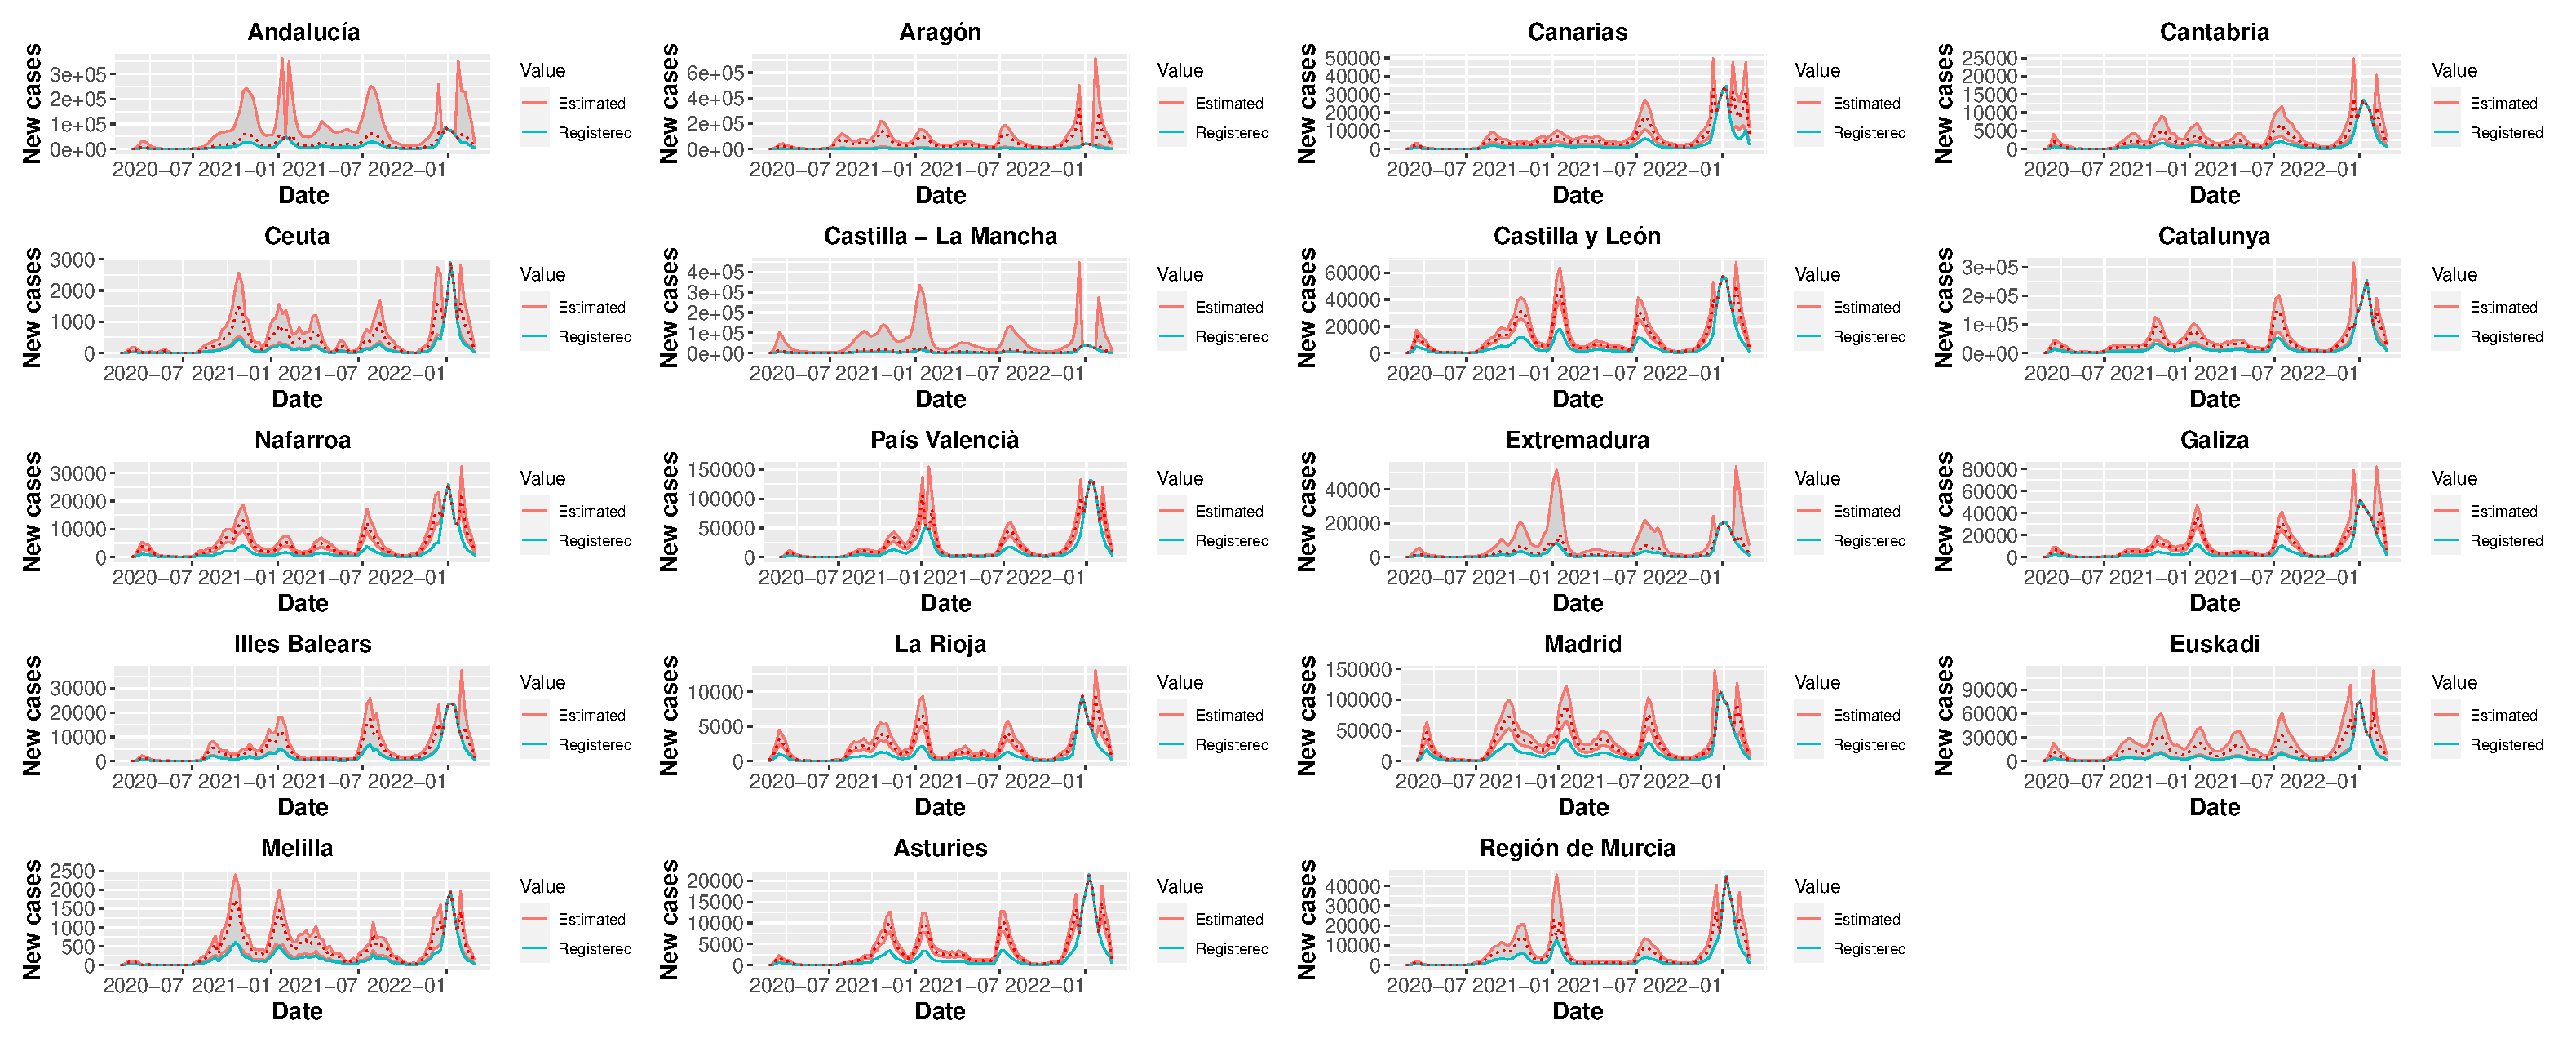
\includegraphics[height=8cm, width=13cm]{morinafig1}
\caption{\label{morina:fig1} Registered and estimated weekly new Covid-19 cases in each Spanish region.}
\end{figure}

In the considered period, the official sources reported 11,056,797 Covid-19 cases in Spain, while the model estimates a total of 25,283,406 cases (only 43.73\% of actual cases were reported). This work also revealed that while the frequency of underreporting is extremely high for all regions (values of $\hat{\omega}$ over 0.90 in all cases), the intensity of this underreporting is not uniform across the considered regions: Arag\'on is the CCAA with highest underreporting intensity ($\hat{q}=0.05$) while Extremadura is the region where the estimated values are closest to the number of reported cases ($\hat{q}=0.50$). Detailed underreported parameter estimates for each region can be found in Table~\ref{morina:tab1}. Although the main impact of the vaccination programmes can be seen in mortality data, the results of this work also showed a significant decrease in the weekly number of cases as well in all CCAA except Arag\'on. Figure~\ref{morina:fig2} represents the estimated and registered processes globally for Spain.

\begin{figure}[!ht]\centering
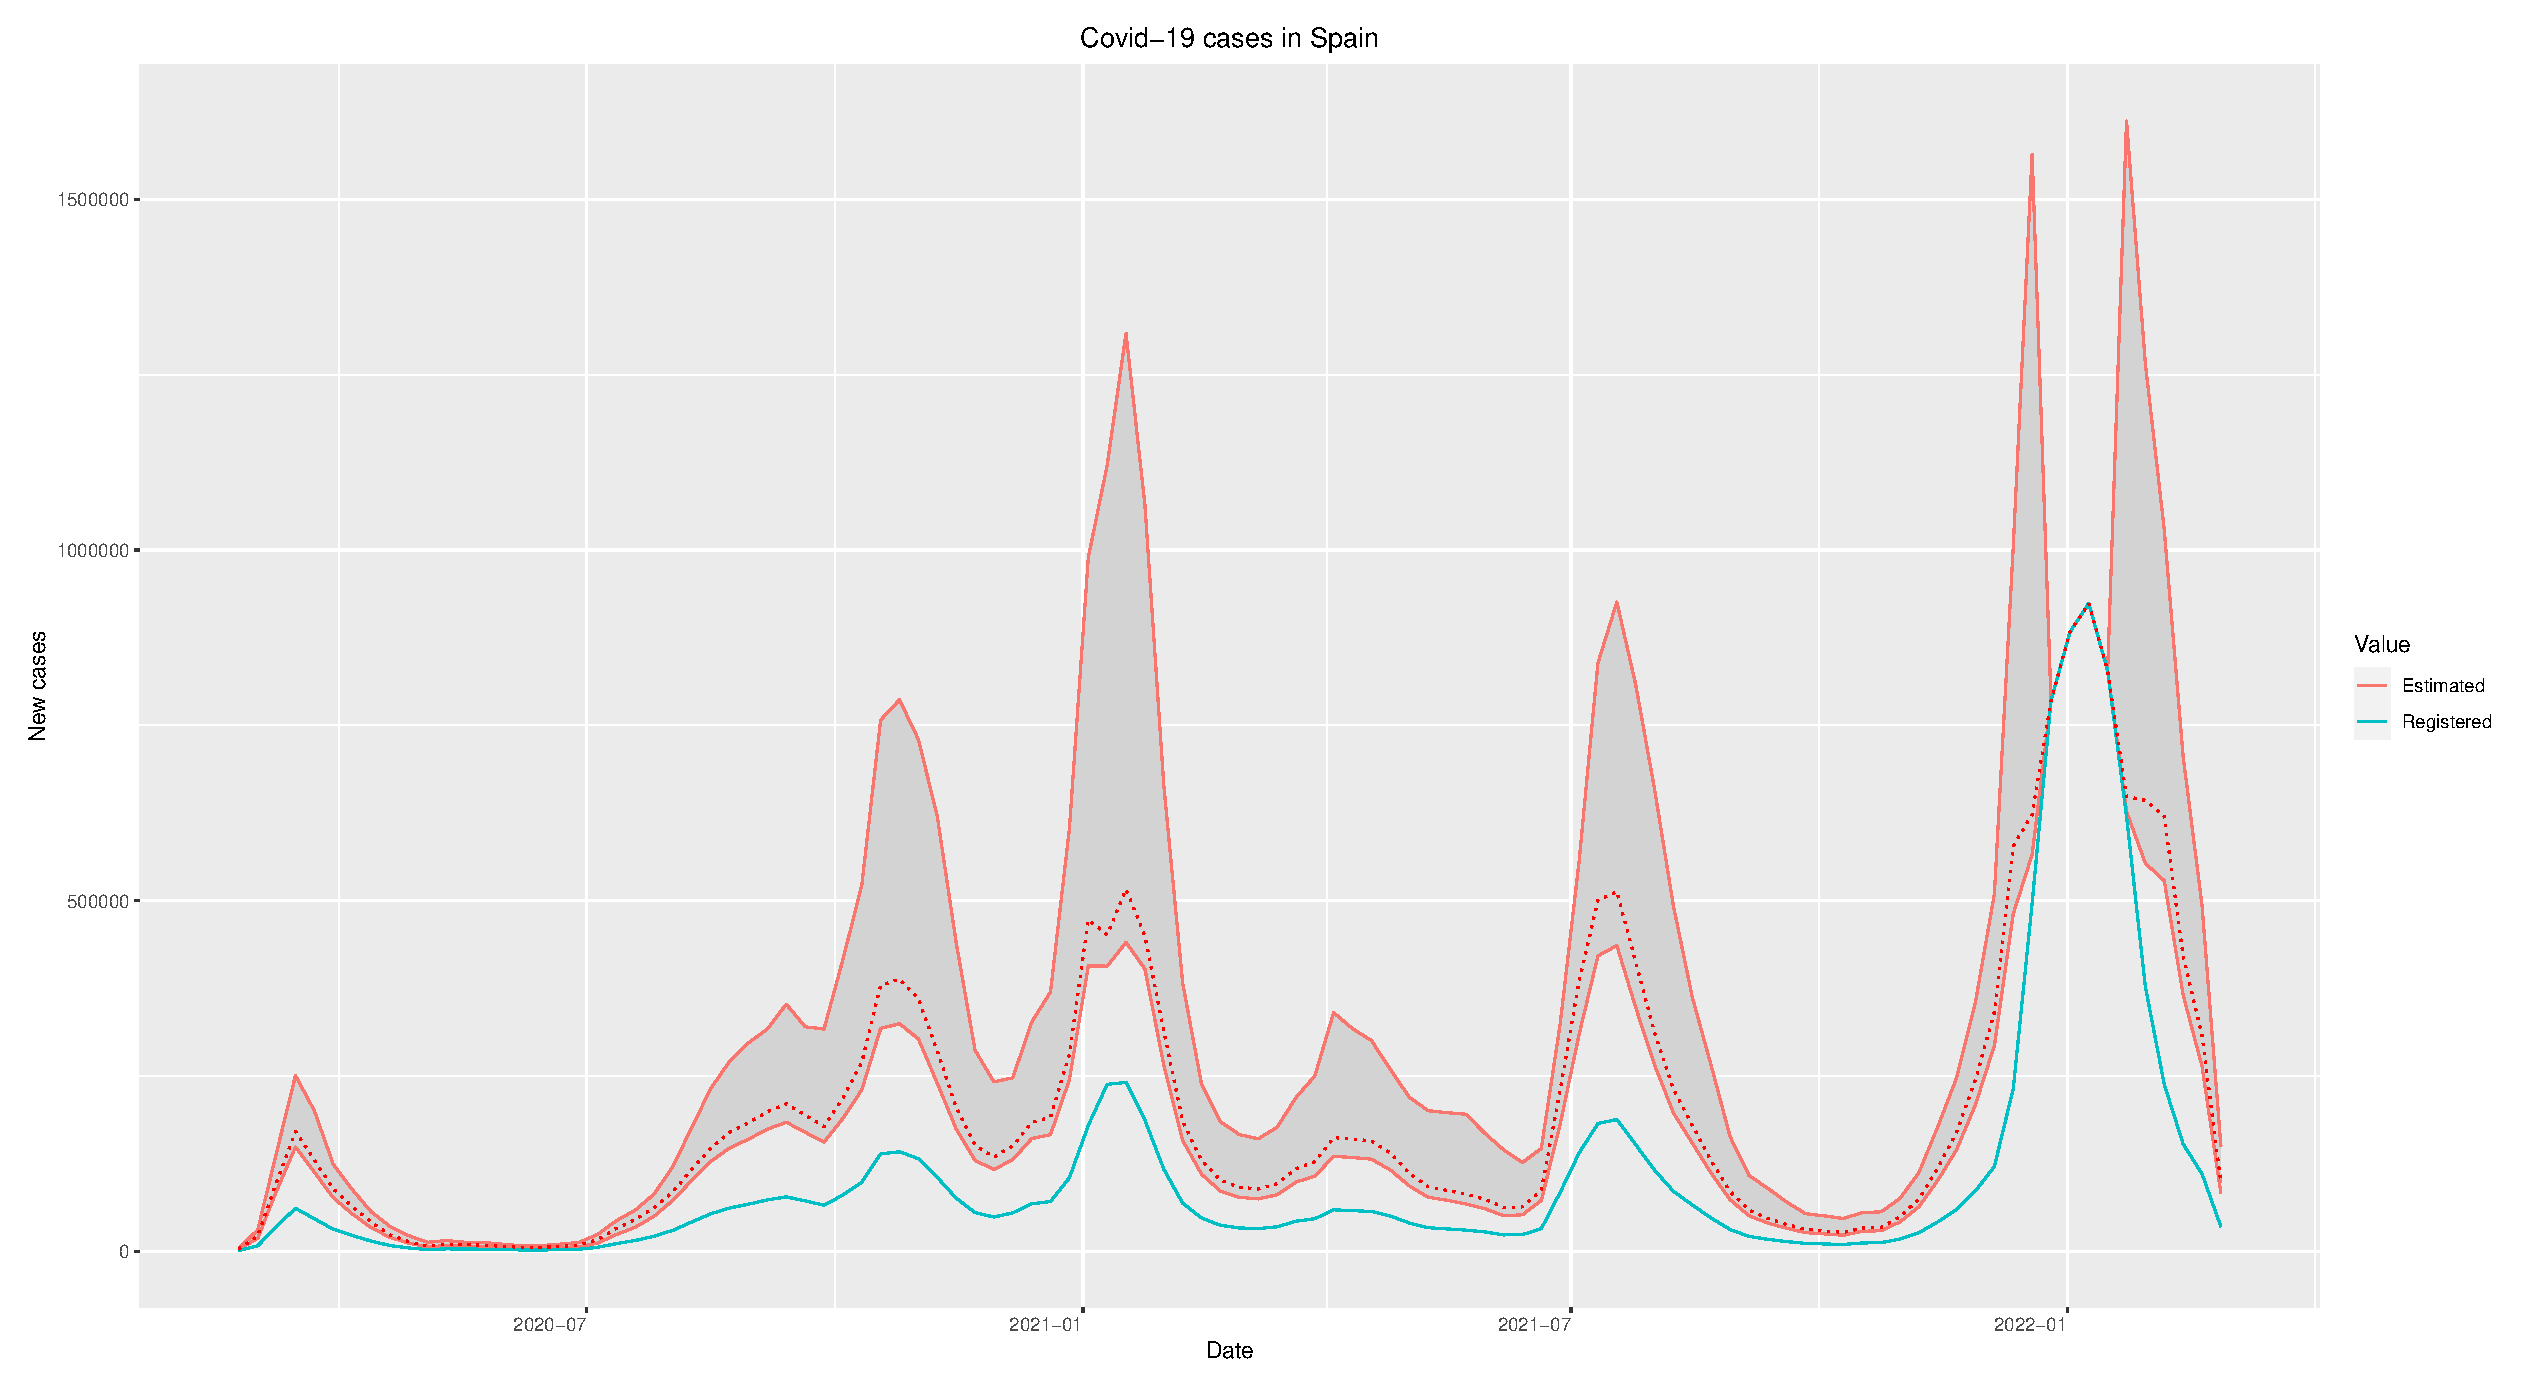
\includegraphics[width=12cm]{morinafig2}
\caption{\label{morina:fig2} Registered and estimated weekly new Covid-19 cases globally in Spain.}
\end{figure}

%***********************************************************************

% Tables can be included at any place in the text.
% As general format, use tables with horizontal lines only
% (i.e., no vertical lines separating columns).
% Start and end each table with a double horizontal line.
% Tables are incorporated using a table environment:

\begin{table}[!ht]\centering
% A caption is put above the table and a label is defined
% to be used for reference to this specific table.
% Use labels which are very unlikely to be used by
% other contributors; for example, use labels starting
% with the surname of the first author.
\caption{\label{morina:tab1} Estimated underreported frequency and intensity for each Spanish region. CI stands for Credible Interval.}
% A table with three columns, where the first is left aligned,
% the second has centred entries, and the third is right aligned,
% is generated as follows (note: if requested, use \cmidrule{} instead of \cline{})
\medskip
\begin{tabular}{ccc}
% First line:
\toprule[0.09 em]
% The body of the table:
Region & Parameter & Estimate (95\% CI) \\
\midrule
\multirow{2}{*}{Andaluc\'ia}  & $\hat{\omega}$  & 0.96 (0.89 - 0.98) \\
                              & $\hat{q}$       & 0.45 (0.41 - 0.51) \\
\cmidrule{1-3}
\multirow{2}{*}{Arag\'on}    & $\hat{\omega}$  & 0.97 (0.97 - 0.98) \\
                             & $\hat{q}$       & 0.05 (0.05 - 0.29) \\
\cmidrule{1-3}
\multirow{2}{*}{Principado de Asturias}    & $\hat{\omega}$  & 0.98 (0.97 - 0.99) \\
                                           & $\hat{q}$       & 0.35 (0.33 - 0.37) \\
\cmidrule{1-3}
\multirow{2}{*}{Cantabria}    & $\hat{\omega}$  & 0.97 (0.95 - 0.99) \\
                              & $\hat{q}$       & 0.31 (0.28 - 0.35) \\
\cmidrule{1-3}
\multirow{2}{*}{Castilla y Le\'on}    & $\hat{\omega}$  & 0.98 (0.96 - 0.99) \\
                                      & $\hat{q}$       & 0.38 (0.34 - 0.40) \\
\cmidrule{1-3}
\multirow{2}{*}{Castilla - La Mancha}    & $\hat{\omega}$  & 0.96 (0.93 - 0.99) \\
                                         & $\hat{q}$       & 0.36 (0.30 - 0.39) \\
\cmidrule{1-3}
\multirow{2}{*}{Canarias}    & $\hat{\omega}$  & 0.98 (0.96 - 0.99) \\
                             & $\hat{q}$       & 0.32 (0.29 - 0.36) \\
\cmidrule{1-3}
\multirow{2}{*}{Catalunya}    & $\hat{\omega}$  & 0.98 (0.96 - 0.99) \\
                               & $\hat{q}$       & 0.35 (0.33 - 0.39) \\
\cmidrule{1-3}
\multirow{2}{*}{Ceuta}    & $\hat{\omega}$  & 0.97 (0.94 - 0.99) \\
                               & $\hat{q}$       & 0.30 (0.27 - 0.35) \\
\cmidrule{1-3}
\multirow{2}{*}{Extremadura}    & $\hat{\omega}$  & 0.90 (0.49 - 0.97) \\
                                & $\hat{q}$       & 0.50 (0.39 - 0.70) \\
\cmidrule{1-3}
\multirow{2}{*}{Galiza}     & $\hat{\omega}$  & 0.98 (0.97 - 0.99) \\
                             & $\hat{q}$       & 0.33 (0.30 - 0.35) \\
\cmidrule{1-3}
\multirow{2}{*}{Illes Balears}    & $\hat{\omega}$  & 0.96 (0.88 - 0.98) \\
                                   & $\hat{q}$       & 0.39 (0.35 - 0.61) \\
\cmidrule{1-3}
\multirow{2}{*}{Regi\'on de Murcia}    & $\hat{\omega}$  & 0.97 (0.92 - 0.99) \\
                                       & $\hat{q}$       & 0.43 (0.38 - 0.48) \\
\cmidrule{1-3}
\multirow{2}{*}{Madrid}      & $\hat{\omega}$  & 0.98 (0.96 - 0.99) \\
                             & $\hat{q}$       & 0.40 (0.36 - 0.42) \\
\cmidrule{1-3}
\multirow{2}{*}{Melilla}    & $\hat{\omega}$  & 0.97 (0.95 - 0.99) \\
                               & $\hat{q}$       & 0.35 (0.32 - 0.38) \\
\cmidrule{1-3}
\multirow{2}{*}{Comunidad Foral de Navarra}    & $\hat{\omega}$  & 0.98 (0.97 - 0.99) \\
                                               & $\hat{q}$       & 0.31 (0.29 - 0.34) \\
\cmidrule{1-3}
\multirow{2}{*}{Euskadi}    & $\hat{\omega}$  & 0.98 (0.96 - 0.99) \\
                               & $\hat{q}$       & 0.30 (0.28 - 0.35) \\
\cmidrule{1-3}
\multirow{2}{*}{La Rioja}    & $\hat{\omega}$  & 0.98 (0.96 - 0.99) \\
                             & $\hat{q}$       & 0.32 (0.29 - 0.35) \\
\cmidrule{1-3}
\multirow{2}{*}{Pa\'is Valenci\`a}    & $\hat{\omega}$  & 0.99 (0.97 - 0.99) \\
                                         & $\hat{q}$       & 0.38 (0.37 - 0.41) \\
% last line:
\bottomrule[0.09 em]
\end{tabular}
\end{table}

% In the text, reference to the Table can be made as follows:
%We refer to Table~\ref{smith:tab1} for a summary of our main results. Have a look to Table~\ref{smith:tab2} for
%an additional example.

%\begin{table}[!ht]\centering
%\caption{\label{smith:tab2} Caption text \textbf{ABOVE} the table.}
%\medskip
%\begin{tabular}{lcr}
% First line:
%\toprule[0.09 em]
% The body of the table:
%  &\multicolumn{2}{c}{Title  for cols 2 -3} \\
%\cmidrule{2-3} %
%Title1 & Title2 & Title3 \\
%\midrule
%& $a$  & $c$ \\
%& $b$  & $d$ \\ %
%\midrule[0 em]
%Total  & $a+b$  & $n$  \\
% last line:
%\bottomrule[0.09 em]
%\end{tabular}
%\end{table}



%***********************************************************************

% Figures can be included at any place in the text.
% The only allowed formats for figures are pdf files.
%
% Please, do not include figures in any other format.
%
% Use file names which are very unlikely to be used by
% other contributors; for example, use file names starting
% with the surname of the first author.
% Figures are incorporated using a figure environment:
% Make sure you specify the extension of the file (pdf)

%Finally a figure (in \verb|.pdf|!)

%\begin{figure}[!ht]\centering
% You can pre-specify the width of the graph:
%\includegraphics[width=8cm]{castelo.pdf}
% Below the figure, a caption is put, and a label is defined
% to be used for reference to this specific figure.
% Use labels which are very unlikely to be used by
% other contributors; for example, use labels starting
% with the surname of the first author.
%\caption{\label{smith:fig1} Caption text \textbf{BELOW} the figure.}
%\end{figure}


% In the text, reference to the Figure can be made as follows:
%We refer to Figure~\ref{smith:fig1} for a~graphical representation.

%***********************************************************************

% Acknowledgments, if needed:
\acknowledgments{Investigation funded by Fundaci\'on MAPFRE.}

%***********************************************************************

% References should be placed in the text in author (year) form.
% The list of references should be placed below IN ALPHABETICAL ORDER.
% (Please follow the format of the examples very tightly).

\references
\begin{description}

\item[An, Z., South, L.F. and Drovandi, C.] (2019). BSL: An R Package for Efficient Parameter
  Estimation for Simulation-Based Models via Bayesian Synthetic Likelihood.
  {\it arXiv preprint}.

\item[Fern{\'{a}}ndez-Fontelo, A., Mori{\~{n}}a, D., Caba{\~{n}}a, A., Arratia, A. and Puig P.] (2020).
  Estimating the real burden of disease under a pandemic situation: The
  SARS-CoV2 case. {\it PLoS ONE}, {\bf 15}, e0242956.

\item[Mori{\~{n}}a, D., Fern{\'{a}}ndez-Fontelo, A., Caba{\~{n}}a, A. and Puig P.] (2021) New
  statistical model for misreported data with application to current public
  health challenges. {\it Scientific Reports}, {\bf 11}, 23321.

\item[Oran, D.P. and Topol, E.J.] (2020). Prevalence of asymptomatic SARS-CoV-2 infection. {\it
  Annals of Internal Medicine}, {\bf 173(5)}, 362\,--\,367.

\item[Price, L.F., Drovandi, C.C., Lee, A. and Nott D.J.] (2018). Bayesian synthetic likelihood. {\it
  Journal of Computational and Graphical Statistics}, {\bf 27(1)},
  1\,--\,11.

\item[Wood S. N.] (2010). Statistical inference for noisy nonlinear ecological dynamic
  systems. {\it Nature}, {\bf 466(7310)}, 1102\,--\,1104.

\end{description}

\end{document}
